% !TeX root = ../diss.tex
\section{Repository Overview}

The majority of my code is in the \texttt{ppl} directory, which contains the core library, unit tests, statistical testing code and some example programs written using the library. The build system dune makes 


I have implemented my ppl as a library (in the \texttt{lib} subdirectory), contained within the module \texttt{Ppl}. This contains several submodules, most importantly the \texttt{Dist} module, which contains the code for representing, creating and combining distributions. 

% TODO: this might change?
The Primitives module contains an type for representing primitive distributions. This type is not abstract, in order to allow users to create their own distributions outside of the ones provided in the module.

The Plot module contains helper functions which wrap around Owl\_plplot, allowing users to easily create visualisations from distributions defined in my ppl.

The \texttt{evaluation} directory contains code to compare my ppl to both hand-written inference procedures, as well as equivalent programs in other PPLs. There are several directories, which each correspond to a particular problem/model, for example the \texttt{hmm} folder for an example of a hidden Markov model.

All code is written in OCaml 4.08, with the main dependencies being Jane Street's \texttt{Core} and \texttt{Owl} \cite{owl}.

\section{Representing Distributions}

As mentioned before, monads are a natural way to represent probability distributions. They allow the output from one distribution (essentially a sample), to be used as if it was of the type that the distribution is defined over. Essentially, the \texttt{bind} operation allows us to 'unwrap' the 'a dist type to allow us to manipulate a value of type 'a. We must then use \texttt{return} to `wrap' the value back into a value of type 'a dist.

Using monads also allows us to define several helper functions which can be used when working with distributions. For example, we can `lift' operators to the \texttt{dist} type, for example allowing us to define adding two distributions over integers or floats using liftM or liftM2. We can also fold lists of distributions using a similar technique.

Using monads also allows the use of the extended let operators introduced in OCaml 4.08. These allow the definition of custom let operators, which mimic do-notation in Haskell. This means that sampling from a distribution (within a model) can be done using the \texttt{let*} operator, and the variable that is bound to can be used as if it were a normal value. The one caveat is that the user must remember to \texttt{return} at the end of the model with whatever variable(s) they want to find the posterior over.

The type signature of bind is \texttt{'a m -> ('a -> 'b m) -> 'b m}, and return is \texttt{'a -> 'a m}, with m being the monad type.

% explain monads here?

However, there are many different underlying data structures which can be used to represent distributions. The simplest is a list of pairs representing a set of values and corresponding probabilities, \texttt{('a * float) list}. This is a very convenient and natural way to represent discrete distributions, with return and bind defined as in listing \ref{lst:monad_plist}. Here, \texttt{return} gives us the distribution with just one value, and bind combines a distribution with a function that takes every element from the initial distribution and applies a function that creates a set of new distributions. The new distributions are then `flattened' and normalised. This approach has been used to create functional probabilistic languages \cite{erwig}, but has several drawbacks, primarily the fact that it cannot be used to represent continuous distributions, and that inference is not efficient - there is no information from the model encoded in this representation, such as how random variables are combined or from what distributions they came from.

% TODO: finish the snippet, write unduplicate properly
\lstinputlisting[language={Caml},caption={Simple Probability Monad},label={lst:monad_plist}]{code_snippets/probmonad_list.ml}

A major problem with this approach is that in flattening distributions, we must make sure that duplicated values are combined, and this approach is $O(n^2)$ when using a list since we must scan up to the length of the entire list for every element. A better option is to use a polymorphic map, which is provided in the Jane Street Core library, and implemented as a balanced tree, significantly improving the time complexity of combining distributions.

\lstinputlisting[language={Caml},caption={Simple Probability Monad using a map},label={lst:monad_pmap}]{code_snippets/probmonad_map.ml}

Although this is not the final data structure I chose for general probabilistic models, it is the one I used for discrete distributions. I also used a Map for the data structure that produced approximations to discrete posterior distributions.

\section{GADT}

% TODO: check this
The structure that I landed on to represent general models is a generalised algebraic data type. GADTs have been used to represent probabilistic models \cite{scibior2015practical} and are widely used to implement interpreters in functional languages. GADTs are similar to ADTs (sum types), in that they have a set of constructors, but the main difference is that these constructors can have type arguments, making sure that programs are well-typed and rejecting invalid programs. The GADT represents a model, and can then be 'interpreted' by a sampler or an inference algorithm. For sampling, I traverse the model, ignoring conditionals to enable forward sampling. For inference, I provide functions which transform the conditional distributions to distributions without any conditional statements, allowing sampling to be performed as normal. Primitive distributions also have a special variant (which takes a different \texttt{primitive} type), since we can find exact the exact pdf/cdf of these distributions, unlike the \texttt{dist} type, which can only be sampled from. The implementation can be seen in listing \ref{lst:gadt1}. The monad functions are also provided, which just construct the corresponding variant in the GADT.

\lstinputlisting[language={Caml},label={lst:gadt1},caption={Representing a probabilistic model using a GADT}]{code_snippets/gadt.ml}

\section{Conditioning}
% https://www.robots.ox.ac.uk/~twgr/assets/pdf/rainforth2017thesis.pdf - section on conditioning, pg.42
The condition variant is used to assign scores to traces, and takes a function which takes an element and returns a float, a `score', which represents how likely that element is. I have also implemented a few helpers to make it easier to condition models. The three main helpers are \texttt{condition}, \texttt{score} and \texttt{observe}, which are all specific cases of the general \texttt{Condition} variant. 

The \texttt{condition} operator is used for hard conditioning, which conditions the model on an observation being true. If true is passed in, then the score assigned is 0, and if false, the score assigned is -infinity.

For soft conditioning, for example an observation that we know comes from a certain distribution, there is an \texttt{observe} function. This function is essential for continuous distributions, since the probability of observing any one value is 0, making hard conditioning redundant.

The \texttt{score} function is similar to the condition operator, except instead of 0, it assigns a particular score (any float) to the trace. An example is %todo.

\section{Primitive Distributions}
In PPLs, users build complex models by composing more simple elementary primitive distributions (ERPs) \cite{pmlr-v15-wingate11a}. These primitive distributions need to have a few operations defined on them, namely \texttt{sample, pdf, cdf} and \texttt{support}.

\section{Forward Sampling}
% https://www.robots.ox.ac.uk/~twgr/assets/pdf/rainforth2017thesis.pdf - sec 7.1, pg 135
In order to perform inference, we will often need to find a prior distribution. For a posterior, $P(\theta\mid x)$, the model written by the user is $P(x\mid\theta)$, and the prior is $P(\theta)$, so finding the prior is the same as disregarding the conditionals (essentially ignoring the data). Since sampling is only difficult in the presence of conditionals, this allows us to sample from the prior using essentially the same sample function. We can also take into account the conditionals, and produce weighted samples, with the weight being the score assigned by each conditional branch, accumulated (by multiplying).

\section{Inference}

Inference is the key motivation behind probabilistic programming. 

Inference can be thought of as a program transformation \cite{scibior2015practical} \cite{Zinkov2016ComposingIA}. In my ppl, this corresponds to a function of type \texttt{'a dist -> 'a dist}. This method allows for the composition of inference algorithms, exemplified in section \ref{sec:pimh}.

Since I have used a trace-based approach, we can characterise the posterior probability of a trace as (from the previous chapter):
% https://www.robots.ox.ac.uk/~twgr/assets/pdf/rainforth2017thesis.pdf - pg.52
$$p(x_{1:N}|y_{1:N})\propto\tilde{p}(y_{1:N},x_{1:N})$$

We can now see how this formula corresponds to a program in my ppl. The example below is a very simple model, which adds two numbers drawn from discrete distributions, and observes a value.

% TODO: write example program, and relate to terms in formula

\subsection{Enumeration} \label{sec:enum}
Enumeration is the simplest way to perform exact inference on probabilistic programs, and essentially consists of computing the joint distribution over all the random variables in the model. This involves enumerating every execution path in the model, in this case performing a depth first search over the \texttt{dist} data structure. For every \texttt{bind} (i.e. every \texttt{let*}), there is a distribution ($d$) and a function from samples to new distributions ($f$). I call this function on every value in the support of the distribution $d$, and then enumerate all the possibilities. The final output is a \texttt{('a * float) list}, which needs to have duplicates removed and then be normalised.

\lstinputlisting[language={Caml},caption={Enumerating all paths through a model},label={lst:enum}]{code_snippets/enumerate.ml}

This method is very naive, and therefore inefficient. Since we essentially take every possible execution trace, we do not exploit structure such as overlapping traces. This can be made slightly more efficient by using algorithms such as belief propagation \cite{belief-prop}, but they still only work on models made up from discrete distributions. Exact inference of this kind only works on models that can be represented as finite networks, and exact inference for Bayesian networks is in fact NP-hard\cite{cooper1990computational}. So instead, most of my project focuses on approximate inference.

\subsection{Rejection Sampling} \label{sec:rej}
\subsection{Importance Sampling} \label{sec:imp}
\subsection{Metropolis Hastings} \label{sec:mh}
\subsection{Particle Filter} \label{sec:pf}
\subsection{Particle Cascade} \label{sec:pc}
\subsection{Particle-Independent Metropolis-Hastings} \label{sec:pimh}

\section{Examples}

\subsection{Sprinkler}
% to show exact inference on discrete model
The sprinkler model is a commonly used example in Bayesian inference due to it's simplicity. It is an example of a \textit{Bayesian network}, and can be visualised as in figure \ref{fig:sprinkler-network}

\begin{figure}[!htb]
	\centering
	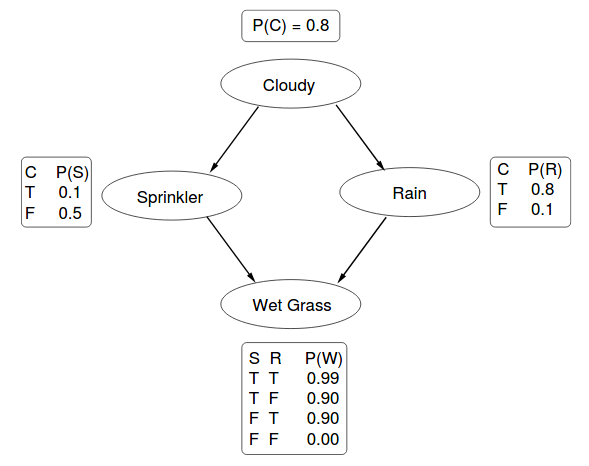
\includegraphics[width=\textwidth]{figs/sprinkler-network.png}
	\caption{Bayesian Network example}
	\label{fig:sprinkler-network}
\end{figure}

\subsection{Biased Coin}
% to show analytically solvable continuous distribution
% include graph of beta compared to computed posterior
Modelling a biased coin shows an example of a very simple model with a continuous posterior that can be calculated analytically\cite{datasci}. 

The model is of a coin that is tossed $n$ times to give $x$ heads. We do not know if the coin is biased or not, and would like to find out the bias, $p$ of the coin, where $p$ is the probability of heads, with $p=0.5$ being an unbiased coin.

To find the posterior, we use an uninformative prior, the uniform. The likelihood model is a binomial.

\begin{align*}
	\Theta\sim Uniform(0,1)\\
	X &\sim Binom(n,\theta)
\end{align}

We then use Bayes' rule to calculate the posterior.
			    
\begin{align*}						
	Pr_{\Theta}(\theta \mid X=x) & = \frac{1}{\kappa}Pr_{\Theta}(\theta)Pr_X(x\mid\theta)    \\ 
	                             & = \frac{1}{\kappa}{{n}\choose{x}}\theta^x(10\theta)^{n-x} \\
	                             & = \frac{1}{\kappa'}\theta^x(1-\theta)^{n-x}               
\end{align}
$$\kappa'=\int_{\phi=0}^1\phi^x(1-\phi)^{n-x}~d\phi$$                        

This results in the posterior, the beta distribution, specifically Beta$(x+1,n-x+1)$. 

The program in my PPL is shown in listing \ref{lst:coin}, and demonstrates setting up the model, performing inference as well as finding the mean of the posterior. The application is to find the chance of the next coin flip landing heads. This example uses $n=10$ and $x=9$, so the mean produced is roughly 0.83, the mean of Beta$(10,2)$.

\lstinputlisting[language={Caml},caption={Coin model},label={lst:coin}]{code_snippets/coin.ml}

\subsection{HMM}
Hidden Markov models are slightly more involved models, where we have a sequence of hidden states, which emit observed states. There are two distributions involved here, the transition distribution, which defines how likely the next state is given the current state, and the emission distribution, which is the 
% use forward-backward to get exact posterior

\subsection{Linear Regression}

\subsection{Dirichlet process}

% Need to show examples which can't be done in graph based thing
% Need to explain why these examples are actually difficult.
% http://www.cs.cmu.edu/~epxing/Class/10708-16/slide/lecture18-DP.pdf
% This is a non-parametric bayesian model - 
% no. of params is infinite, grows with size of dataset

\section{Statistical tests}
I had to implement a number of statistical tests in order to test the correctness of the output distribution. These tests are known as goodness-of-fit tests, and 

\section{Visualisations}
Visualising the output distributions from inference can be done using the \texttt{Owl\_plplot} module, which allows plotting directly from OCaml, rather than having to interface with other programs manually.